\documentclass[12pt]{article}
\setlength{\oddsidemargin}{0in}
\setlength{\evensidemargin}{0in}
\setlength{\textwidth}{6.5in}
\setlength{\parindent}{0in}
\setlength{\parskip}{\baselineskip}

\usepackage{amsmath,amsfonts,amssymb,bm,graphics,pgfplots,framed,dsfont}
\usepackage[scale=0.75,top=1cm,bottom=3cm]{geometry}

\begin{document}

\textbf{Minh Anh Nguyen }\\
\textbf{Calculus 1 Assignment-7}\\
\textbf{Section: 04}\\
\textbf{TA's name: Arthur Huey}

\hrulefill

Section 3.4:

\begin{enumerate}
    \setcounter{enumi}{2}
    \item For the function $f$ whose graph is given, state the following.
    \begin{center}
        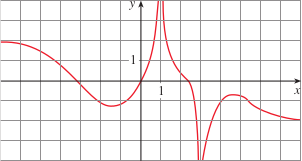
\includegraphics{img/img-0.png}
    \end{center}
    \begin{enumerate}
        \item \[\boxed{\lim_{x \to \infty } f(x) = -2}\]
        \item \[\boxed{\lim_{x \to -\infty} f(x) = 2}\]
        \item \[\boxed{\lim_{x \to 1} f(x) = \infty}\]
        \item \[\boxed{\lim_{x \to 3} f(x) = -\infty}\]
        \item The equations of the asymptotes
        \[\boxed{x = 1, x = 3, y = -2, y = 2}\]
    \end{enumerate}
    \setcounter{enumi}{7}
    \item Evaluate the limit and justify each step by indicating the appropriate properties of limits.
    \[\lim_{x \to \infty} \sqrt{\frac{9x^3+8x-4}{3-5x+x^3}}\]
    \[= \lim_{x \to \infty} \sqrt{\frac{x^3(9+8/x^2-4/x^3)}{x^3(3/x^3-5/x^2+1)}}\]
    \[= \lim_{x \to \infty} \sqrt{\frac{9+8/x^2-4/x^3}{3/x^3-5/x^2+1}}\]
    \[= \sqrt{\frac{9+0-0}{0-0+1}}\]
    \[\boxed{= \sqrt{9} = 3}\]
    \setcounter{enumi}{10}
    \item Find the limit or show that it does not exist.
    \[\lim_{t \to -\infty} \frac{3t^2 + t}{t^3 -4t + 1}\]
    \[= \lim_{t \to -\infty} \frac{t^2(3 + 1/t)}{t^3(1 -4/t^2 + 1/t^3)}\]
    \[= \lim_{t \to -\infty} \frac{(3 + 1/t)}{t(1 -4/t^2 + 1/t^3)}\]
    \[\boxed{= 0}\]
    \setcounter{enumi}{17}
    \item Find the limit or show that it does not exist.
    \[\lim_{t \to \infty}\frac{t+3}{\sqrt{2t^2-1}}\]
    \[=\lim_{t \to \infty}\frac{t(1+3/t)}{t\sqrt{2-1/t^2}}\]
    \[=\lim_{t \to \infty}\frac{1+3/t}{\sqrt{2-1/t^2}}\]
    \[=\frac{1+0}{\sqrt{2-0}}\]
    \[\boxed{=\frac{1}{\sqrt{2}}}\]
    \setcounter{enumi}{25}
    \item Find the limit or show that it does not exist.
    \[=\lim_{x \to -\infty}(\sqrt{4x^2 + 3x} + 2x)\]
    \[=\lim_{x \to -\infty}(|x|\sqrt{4 + 3/x} + 2x)\]
    Because $x$ is approaching to $-\infty$. $|x| = -x$.
    \[=\lim_{x \to -\infty}(-x\sqrt{4 + 3/x} + 2x)\]
    \[=\lim_{x \to -\infty}x(-\sqrt{4 + 3/x} + 2)\]
    \[=-\infty(-2 + 2)\]
    \[=-\infty(0)\]
    \[\boxed{=0}\]
    \newpage
    \setcounter{enumi}{27}
    \item Find the limit or show that it does not exist.
    \[\lim_{x \to \infty}(x - \sqrt{x})\]
    \[=\lim_{x \to \infty}x(1 - 1/\sqrt{x})\]
    \[=\infty(1 - 0)\]
    \[\boxed{=\infty}\]
    \setcounter{enumi}{30}
    \item Find the limit or show that it does not exist.
    \[\lim_{x\to \infty}x\sin\frac{1}{x}\]
    \[=\infty\sin 0\]
    \[\boxed{=0}\]
    \setcounter{enumi}{36}
    \item Find the horizontal and vertical asymptotes of each curve. You may want to use a graphing calculator (or computer) to check your work by graphing the curve and estimating the asymptotes.
    \[y = \frac{2x^2 + x - 1}{x^2 + x - 2}\]
    Horizontal Asymptotes:
    \[\lim_{x\to \infty}\frac{2x^2 + x - 1}{x^2 + x - 2}\]
    \[=\lim_{x\to \infty}\frac{x^2(2 + 1/x - 1/x^2)}{x^2(1 + 1/x - 2/x^2)}\]
    \[=\lim_{x\to \infty}\frac{2 + 1/x - 1/x^2}{1 + 1/x - 2/x^2}\]
    \[\boxed{=2}\]
    \[\lim_{x\to -\infty}\frac{2x^2 + x - 1}{x^2 + x - 2}\]
    \[=\lim_{x\to -\infty}\frac{x^2(2 + 1/x - 1/x^2)}{x^2(1 + 1/x - 2/x^2)}\]
    \[=\lim_{x\to -\infty}\frac{2 + 1/x - 1/x^2}{1 + 1/x - 2/x^2}\]
    \[\boxed{=2}\]
    \[\boxed{y = 2}\]
    Vertical Asymptotes;
    \[x^2 + x - 2 = 0\]
    \[(x-1)(x+2) = 0\]
    \[\boxed{x=1\text{ or }x=-2}\]
    \[\boxed{x = 1, x = -2}\]
    \newpage
    \setcounter{enumi}{53}
    \item Find the limits as $x \to \infty$ and as $x \to -\infty$. Use this information, together with intercepts, to give a rough sketch of the graph as in Example 11.
    \[y = x^3(x + 2)^2(x-1)\]
    \[\lim_{x\to \infty}x^3(x + 2)^2(x-1)\]
    \[\boxed{=\infty}\]
    ~\\~
    \[\lim_{x\to -\infty}x^3(x + 2)^2(x-1)\]
    \[\boxed{= \infty}\]
    \begin{figure}[!h]      
        \begin{framed}
            \centering  
            \begin{tikzpicture}
                \begin{axis}[
                    axis lines = middle,
                    xlabel = $x$,
                    ylabel = {$f(x)$},
                    samples = 100,
                    domain = -4:2,
                    ymin=-10, ymax=10,
                ]
                \addplot[
                    thick,
                    blue,
                ]{x^3*(x + 2)^2*(x - 1)};
                \end{axis}
            \end{tikzpicture}
        \end{framed}
        \end{figure}
    \setcounter{enumi}{58}
    \item Sketch the graph of a function that satisfies all of the given conditions.
\end{enumerate}
\newpage
Section 3.5:
\begin{enumerate}
\setcounter{enumi}{4}
    \item Use the guidelines of this section to sketch the curve.
    \[y = x(x-4)^3 = x(x^3 - 3x^2 \times 4 + 3x \times 4^2 - 4^3)\]
    \[y = x(x^3 - 12x^2 + 48x - 64) = x^4 - 12x^3 + 48x^2 - 64x\]
    \begin{enumerate}
        \item Domain: $(-\infty, \infty)$
        \item Intercepts:
        \[f(0) = 0(0-4)^3 = 0\]
        \[y-\text{intercepts are 0}\]
        \[f(x) = x(x-4)^3 = 0\]
        \[x-\text{intercepts are 0 and 4}\]
        \item Symmetry:
        \[f(-x) = (-x)^4 - 12(-x)^3 + 48(-x)^2 - 64(-x)\]
        \[f(-x) = x^4 + 12x^3 + 48x^2 + 64x\]
        The function is not odd nor even.
        \item Asymptotes:\\
        Since the function is a polynomial function. It will be defined everywhere and has no vertical asymptote.
        \[\lim_{x \to \infty} f(x) = \lim_{x \to \infty} x^4 - 12x^3 + 48x^2 - 64x = \infty\]
        \[\lim_{x \to -\infty} f(x) = \lim_{x \to -\infty} x^4 - 12x^3 + 48x^2 - 64x = \infty\]
        The function also doesn't have horizontal asymptote.
        \item Intervals of Increase or Decrease:
        \[f'(x) = 4x^3 - 36x^2 + 96x - 64 = 0\]
        \[x = 1 \text{ or } x = 4\]
        \begin{center}
            \begin{tabular}{c c c c c c c c}
                $x$ & $-\infty$ & ~ & 1 &  & 4 & & $\infty$ \\ 
                \hline 
                $f^\prime (x)$ & & -- & 0 & + & 0 & + & \\ 
                \hline 
                $f(x)$ & ~ & $\downarrow$ & -27 & $\uparrow$ & 0 & $\uparrow$ & \\ 
            \end{tabular}    
        \end{center}
        The function f(x) increases on the intervals $(1,4)$ and $(4, \infty)$.\\
        The function f(x) decreases on the interval $(-\infty, 1)$.
        \item Local Maximum and Minimum Values:\\
        Local Minimum Values is $f(1) = -27$.
        \item Concavity and Points of Inflection:
        \[f''(x) = 12x^2 - 72x + 96 = 0\]
        \[x = 2 \text{ or } x = 4\]
        \begin{center}
            \begin{tabular}{c c c c c c c c}
                $x$ & $-\infty$ & ~ & 2 &  & 4 & & $\infty$ \\ 
                \hline 
                $f^{\prime\prime} (x)$ & ~ & + & 0 & -- & 0 & + \\ 
            \end{tabular}    
        \end{center}
        The function f(x) is concave up on the intervals $(-\infty, 2)$ and $(4, \infty)$.\\
        The function f(x) is concave down on the intervals $(2,4)$.\\
        Points of Inflection are (2, 16) and (4, 0).
        \item Sketch the graph:
        \begin{figure}[!h]
            \centering
            \begin{framed}
                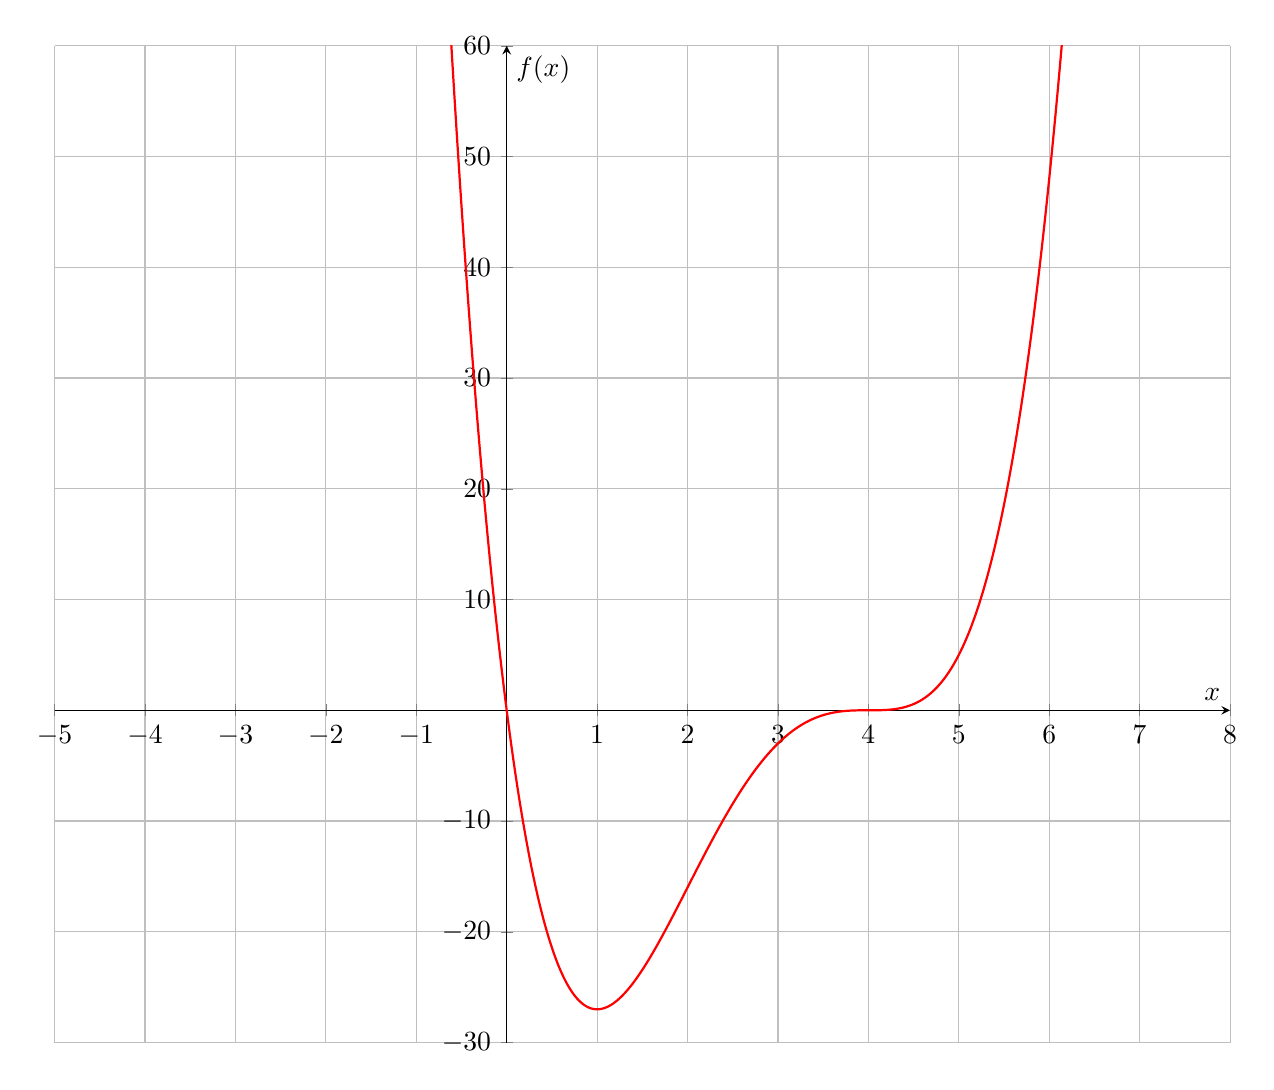
\begin{tikzpicture}
                    \begin{axis}[
                        axis lines = center,
                        xlabel = \(x\),
                        ylabel = {\(f(x)\)},
                        xmin = -5, xmax = 8,  % Adjusted the domain
                        ymin = -30, ymax = 60,  % Adjusted the range
                        samples = 1000,
                        domain = -5:10,  % Updated domain
                        grid = both,  % Optional: adds a grid
                        width = \linewidth,  % Optional: makes the plot fill the width
                    ]
                    \addplot [
                        color = red,
                        thick,  % Optional: thickens the curve
                    ]
                    {x*(x - 4)^3};  % Corrected function
                    \end{axis}
                \end{tikzpicture}
            \end{framed}
        \end{figure}
    \end{enumerate}
    \setcounter{enumi}{8}
    \item Use the guidelines of this section to sketch the curve.
    \[y = \frac{2x+3}{x+2}\]
    \begin{enumerate}
        \item Domain:
            \[x + 2 \neq 0\]
            \[x \neq -2\]
        Hence, the domain of f(x) is: $\mathds{R} \setminus \{-2\}$ 
        \item Intercepts:
            \[f(0) = \frac{2\times 0 + 3}{0 + 2} = \frac{3}{2}\]
            \[f(x) = \frac{2x+3}{x+2} = 0\]
            \[x = -\frac{3}{2}\]
            The y-intercepts of the function is $\frac{3}{2}$.\\
            The x-intercepts of the function is $-\frac{3}{2}$.
        \item Symmetry:
            \[f(-x) = \frac{2(-x)+3}{(-x)+2}\]
            \[f(-x) = \frac{-2x+3}{-x+2}\]
            The function is not odd nor even.
        \item Asymptotes:
            \[\lim_{x \to -2^-} \frac{2x+3}{x+2} = \infty\] 
            \[\lim_{x \to -2^+} \frac{2x+3}{x+2} = -\infty\] 
            The function has a vertical asymptote x = -2.
            \[\lim_{x \to \infty} f(x) = \lim_{x \to \infty} \frac{2x+3}{x+2} = \lim_{x \to \infty} \frac{x(2+3/x)}{x(1+2/x)} 
            = \lim_{x \to \infty} \frac{2+3/x}{1+2/x} = \frac{2 + 0}{1 + 0} = 2\]
            \[\lim_{x \to -\infty} f(x) = \lim_{x \to -\infty} \frac{2x+3}{x+2} = \lim_{x \to -\infty} \frac{x(2+3/x)}{x(1+2/x)} = \lim_{x \to -\infty} \frac{2+3/x}{1+2/x} = \frac{2 + 0}{1 + 0} = 2\]
            The function has a horizontal asymptote y = 2.
        \item Intervals of Increase or Decrease:
            \[f'(x) = \frac{(2x+3)'(x+2)-(x+2)'(2x+3)}{(x+2)^2}\]
            \[f'(x) = \frac{2(x+2)-(2x+3)}{(x+2)^2}\]
            \[f'(x) = \frac{2x+4-2x-3}{(x+2)^2}\]
            \[f'(x) = \frac{1}{(x+2)^2} > 0 \text{ } \forall x \in (\mathds{R} \setminus \{-2\}) \]
            Hence, the function always increases on the domain $\mathds{R} \setminus \{-2\}$.
        \item Local Maximum and Minimum Values:\\
            The function doesn't have any local maximum nor minimum.
        \item Concavity and Points of Inflection:
            \[f''(x) = -\frac{[(x+2)^2]'}{(x+2)^4}\]
            \[f''(x) = -\frac{2(x+2)}{(x+2)^4}\]
            \[f''(x) = -\frac{2}{(x+2)^3}\]
            \begin{center}
                \begin{tabular}{c c c c c c c c}
                    $x$ & $-\infty$ & ~ & -2 & ~ & $\infty$ \\ 
                    \hline 
                    $f^{\prime\prime} (x)$ & ~ & + & 0 & -- \\ 
                \end{tabular}    
            \end{center}
            The function f(x) is concave up in the interval $(-\infty, -2)$.\\
            The function f(x) is concave up in the interval $(-2, \infty)$.\\
        \item Sketch the graph:
            \begin{figure}[!h]
                \centering
                \begin{framed}
                    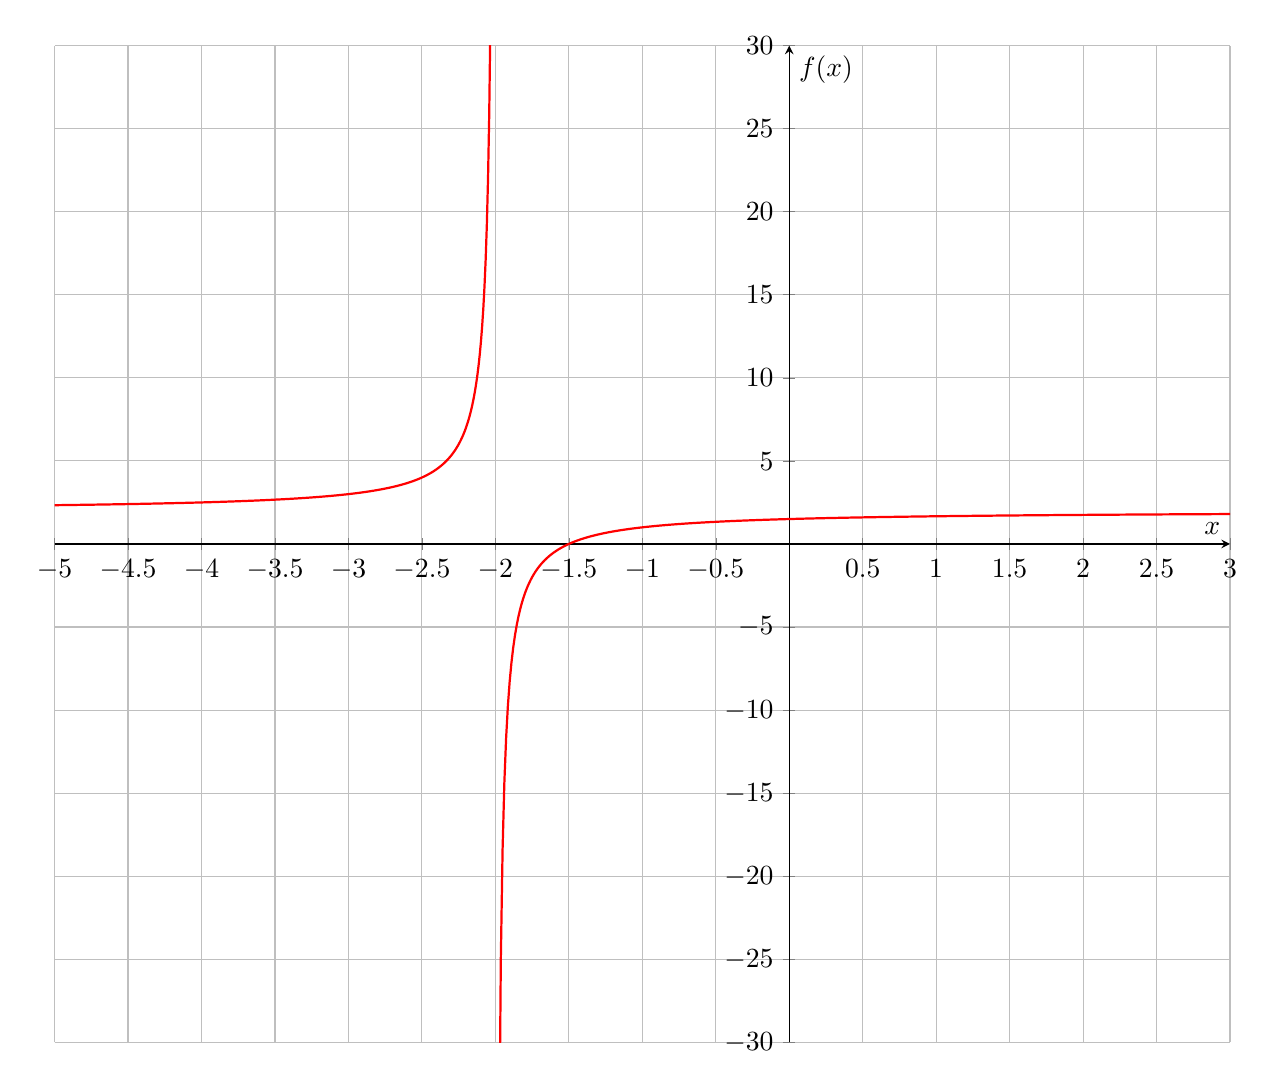
\begin{tikzpicture}
                        \begin{axis}[
                            axis lines = center,
                            xlabel = \(x\),
                            ylabel = {\(f(x)\)},
                            xmin = -5, xmax = 3,  % Adjusted the domain
                            ymin = -30, ymax = 30,  % Adjusted the range
                            samples = 1000,
                            domain = -5:10,  % Updated domain
                            grid = both,  % Optional: adds a grid
                            width = \linewidth,  % Optional: makes the plot fill the width
                        ]
                        \addplot [
                            domain=-10:-2.001, 
                            color = red,
                            thick,  % Optional: thickens the curve
                        ]
                        {(2*x+3)/(x+2)};  % Corrected function
                        \addplot [
                            domain=-1.999:10, 
                            color = red,
                            thick,  % Optional: thickens the curve
                        ]
                        {(2*x+3)/(x+2)};
                        \end{axis}
                    \end{tikzpicture}
                \end{framed}
            \end{figure}
    \end{enumerate}
    \setcounter{enumi}{20}
    \item Use the guidelines of this section to sketch the curve.
    \[y = (x-3)\sqrt{x}\]
    \begin{enumerate}
        \item Domain:
            \[x \geq 0\]
        The domain of the function f(x) is $[0,\infty)$.
        \item Intercepts:
            \[f(0) = (0 - 3)\sqrt{0} = 0\]
            \[f(x) = (x-3)\sqrt{x} = 0\]
            \[(x-3)\sqrt{x} = 0\]
            \[x = 0 \text{ or } x = 3\]
            The y-intercept of the function is 0.\\
            The x-intercepts of the function are 0 and 3.
        \item Symmetry:\\
            Because the function has the domain $[0,\infty)$ so this function is not symmetrical.
        \item Asymptotes:
            \[\lim_{x \to \infty} f(x) = \lim_{x \to \infty} (x-3)\sqrt{x} = \infty \]
            \[\lim_{x \to -\infty} f(x) \text{ is undefined.}\] 
            So the function doesn't have any horizontal nor vertical asymptote.
        \item Interval of Increase or Decrease:
            \[f'(x) = (x-3)'\sqrt{x} + (x-3)\sqrt{x}'\]
            \[f'(x) = \sqrt{x} + \frac{x-3}{2\sqrt{x}}\]
            \[f'(x) = \frac{2x + x-3}{2\sqrt{x}}\]
            \[f'(x) = \frac{3x-3}{2\sqrt{x}} = 0\]
            \[x = 1\]
            \begin{center}
                \begin{tabular}{c c c c c c c c}
                    $x$  & 0 & ~ &1 & ~ & $\infty$ \\ 
                    \hline 
                    $f^{\prime} (x)$ & $||$ & -- & 0 & + \\ 
                    \hline 
                    $f(x)$ & 0 & $\downarrow$ & -2 & $\uparrow$ & \\ 
                \end{tabular}    
            \end{center}
            Hence, the function f increases on the interval $(1,\infty)$.\\
            The function f decreases on the interval $(0,1)$.
        \item Local Maximum and Minimum Values:\\
            The function f has local minimum at x = 1, f(1) = -2.
        \item Concavity and Inflection Point
            \[f''(x) = \frac{(3x-3)'2\sqrt{x} - (2\sqrt{x})'(3x-3)}{4x}\]
            \[f''(x) = \frac{6\sqrt{x} - \frac{1}{\sqrt{x}}(3x-3)}{4x}\]
            \[f''(x) = \frac{6x - 3x + 3}{4x\sqrt{x}}\]
            \[f''(x) = \frac{3x + 3}{4x\sqrt{x}} = 0\]
            \[x = -1\]
            \begin{center}
                \begin{tabular}{c c c c c c c c}
                    $x$ & $-\infty$ & ~ & -1 & ~ & 0 & ~ &$\infty$ \\ 
                    \hline 
                    $f^{\prime\prime} (x)$ & ~ & ~ & ~ & ~ & $||$ & + \\ 
                \end{tabular}    
            \end{center}
            Hence, the function is concave up on the interval $(0,\infty)$
        \newpage
        \item Sketch the graph:
        \begin{figure}[!h]
            \centering
            \begin{framed}
                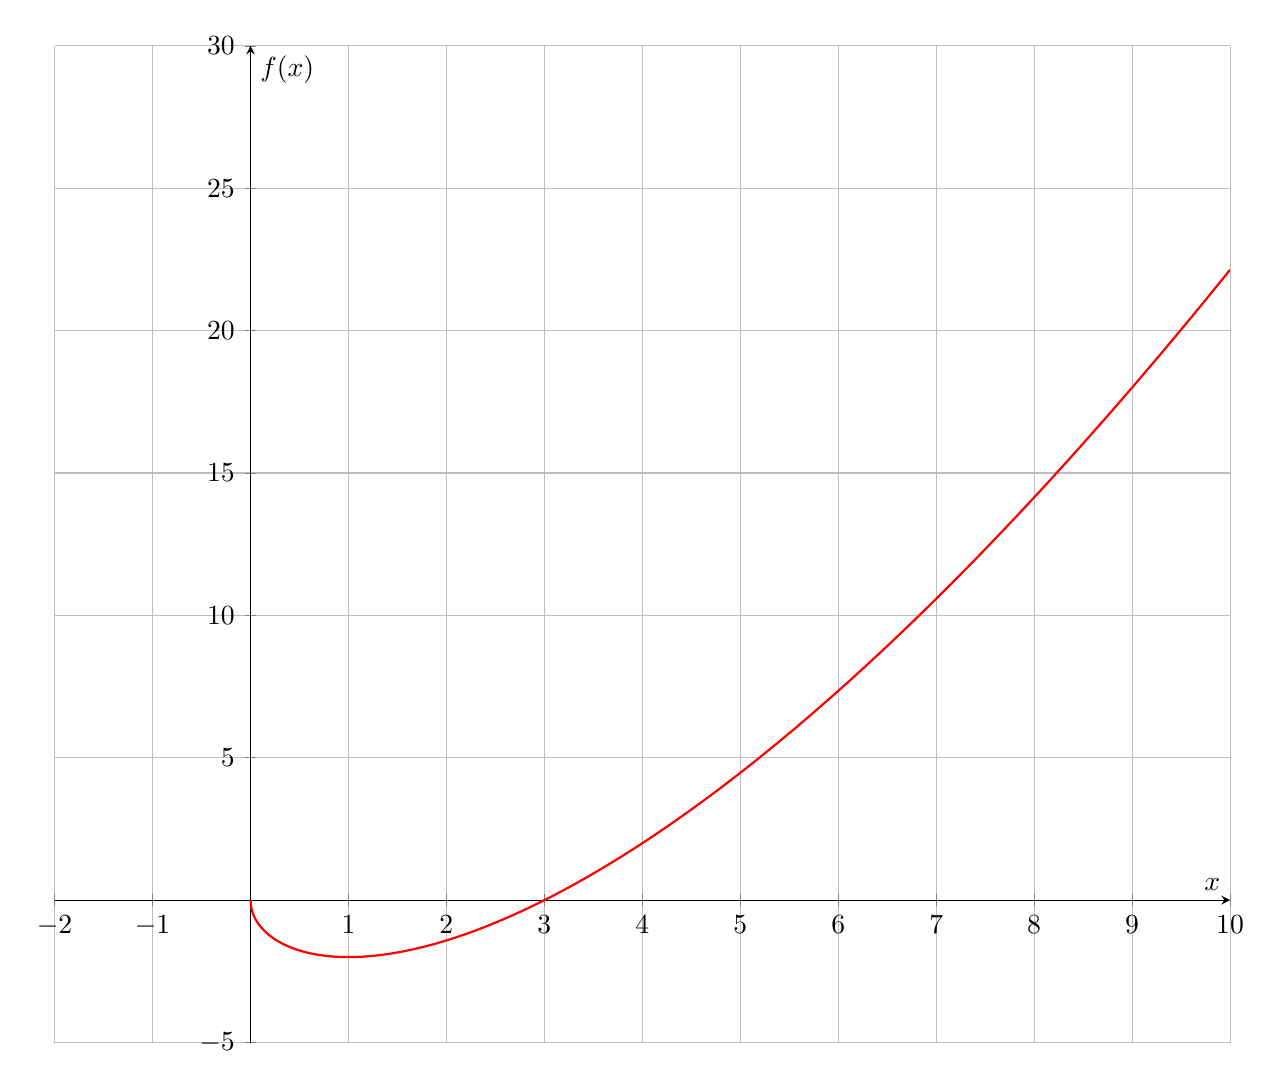
\begin{tikzpicture}
                    \begin{axis}[
                        axis lines = center,
                        xlabel = \(x\),
                        ylabel = {\(f(x)\)},
                        xmin = -2, xmax = 10,  % Adjusted the domain
                        ymin = -5, ymax = 30,  % Adjusted the range
                        samples = 1000,
                        domain = -5:10,  % Updated domain
                        grid = both,  % Optional: adds a grid
                        width = \linewidth,  % Optional: makes the plot fill the width
                    ]
                    \addplot [
                        domain=0:10, 
                        color = red,
                        thick,  % Optional: thickens the curve
                    ]
                    {(x-3)*sqrt(x)};
                    \end{axis}
                \end{tikzpicture}
            \end{framed}
        \end{figure}
    \end{enumerate}
    \setcounter{enumi}{27}
    \item Use the guidelines of this section to sketch the curve.
        \[y = \frac{x}{\sqrt{x^2 - 1}}\]
        \begin{enumerate}
            \item Domain:
                \[x^2 - 1 > 0\]
                \[x^2 > 1\]
                \[x < 1\text{ or } x > 1\]
                Hence, the domain of the function is $(-\infty,1)\cup (1, \infty)$.
            \item Intercepts:
                \[f(0) = \frac{0}{\sqrt{0^2 - 1}} \text{ is not defined}\]
                \[f(x) = \frac{x}{\sqrt{x^2 - 1}} = 0\]
                \[\frac{x}{\sqrt{x^2 - 1}} = 0 \text{ doesn't have any solution.}\]
                Hence, there is no x nor y intercept.
                \newpage
            \item Symmetry:
                \[f(-x) = \frac{-x}{\sqrt{(-x)^2 - 1}} = -\frac{x}{\sqrt{x^2 - 1}}\]
                Hence, $f(-x) = -f(x)$. The graph is odd.
            \item Asymptotes:
                \[\lim_{x \to 1^+} f(x) = \lim_{x \to 1^+} \frac{x}{\sqrt{x^2 - 1}} = \lim_{x \to 1^+} \frac{x}{|x|\sqrt{1 - 1/x^2}} \]
                Since x $>$ 1 and is positive. 
                \[\lim_{x \to 1^+} \frac{1}{\sqrt{1 - 1/x^2}} = \infty\]
                ~\\~\\
                \[\lim_{x \to -1^-} f(x) = \lim_{x \to -1^-} \frac{x}{\sqrt{x^2 - 1}} = 
                \lim_{x \to -1^-} \frac{x}{|x|\sqrt{1 - 1/x^2}}\]
                Since x $<$ 1 and is negative. 
                \[\lim_{x \to -1^-} \frac{-1}{\sqrt{1 - 1/x^2}} = -\infty\]
                ~\\~\\
                \[\lim_{x \to \infty} f(x) = \lim_{x \to \infty} \frac{x}{\sqrt{x^2 - 1}} =
                \lim_{x \to \infty} \frac{1}{\sqrt{1 - 1/x^2}} = \lim_{x \to \infty} \frac{x}{|x|\sqrt{1 - 1/x^2}}\]
                Since x to $\infty$ is positive.
                \[\lim_{x \to \infty} \frac{1}{\sqrt{1 - 1/x^2}} = 1\]
                ~\\~\\
                \[\lim_{x \to -\infty} f(x) = \lim_{x \to -\infty} \frac{x}{\sqrt{x^2 - 1}} = \lim_{x \to -\infty} \frac{-1}{\sqrt{1 - 1/x^2}} = \lim_{x \to -\infty} \frac{x}{|x|\sqrt{1 - 1/x^2}}\]
                Since x to $-\infty$ is negative.
                \[\lim_{x \to -\infty} -\frac{1}{\sqrt{1 - 1/x^2}} = -1\]
                Hence, the vertical asymptotes of the function are x = -1, x = 1.\\
                The horizontal asymptotes of the function are y = -1, y = 1.
            \item Intervals of Increase or Decrease:
                \[f'(x) = \frac{x'\sqrt{x^2-1}-(\sqrt{x^2-1})'x}{(x^2 - 1)}\]
                \[f'(x) = \frac{\sqrt{x^2-1}-\frac{x}{\sqrt{x^2-1}}x}{(x^2 - 1)}\]
                \[f'(x) = \frac{x^2-1-x^2}{\sqrt{x^2-1}(x^2 - 1)}\]
                \[f'(x) = \frac{-1}{\sqrt{x^2-1}(x^2 - 1)} < 0 \text{~} \forall x \in [(-\infty,1)\cup (1, \infty)]\]
                Hence, the function decreases on its interval $(-\infty,1)\cup (1, \infty)$.
            \item Local Maximum and Minimum Values:\\
                The function doesn't have any maximum or minimum values since it always decreases.
            \item Concavity and Inflection Point:
                \[f''(x) = - \frac{(\sqrt{x^2-1}(x^2 - 1))'}{(x^2 - 1)^3}\]
                \[f''(x) = - \frac{\frac{x}{\sqrt{x^2-1}}(x^2 - 1) + 2x\sqrt{x^2-1}}{(x^2 - 1)^3}\]
                \[f''(x) = - \frac{x(x^2 - 1) + 2x(x^2-1)}{\sqrt{x^2-1}(x^2 - 1)^3}\]
                \[f''(x) = - \frac{x^3 - x + 2x^3 - 2x}{\sqrt{x^2-1}(x^2 - 1)^3}\]
                \[f''(x) = - \frac{3x^3 - 3x}{\sqrt{x^2-1}(x^2 - 1)^3} = 0\]
                \[x = 0 \text{ or } x = \pm 1\]\\~
                \begin{center}
                    \begin{tabular}{c c c c c c c c c c}
                        $x$ & $-\infty$ & ~ & -1 & ~ & 0 & ~ & 1 & ~ & $\infty$ \\ 
                        \hline 
                        $f^{\prime\prime} (x)$ & ~ & -- & $||$ & ~ & 0 & ~ & $||$ & + \\ 
                    \end{tabular}    
                \end{center}
                Hence, the function is concave up on the interval $(1, \infty)$.\\
                The function is concave down on the interval $(-\infty, -1)$.
            \newpage
            \item Sketch the graph:
            \begin{figure}[!h]
                \centering
                \begin{framed}
                    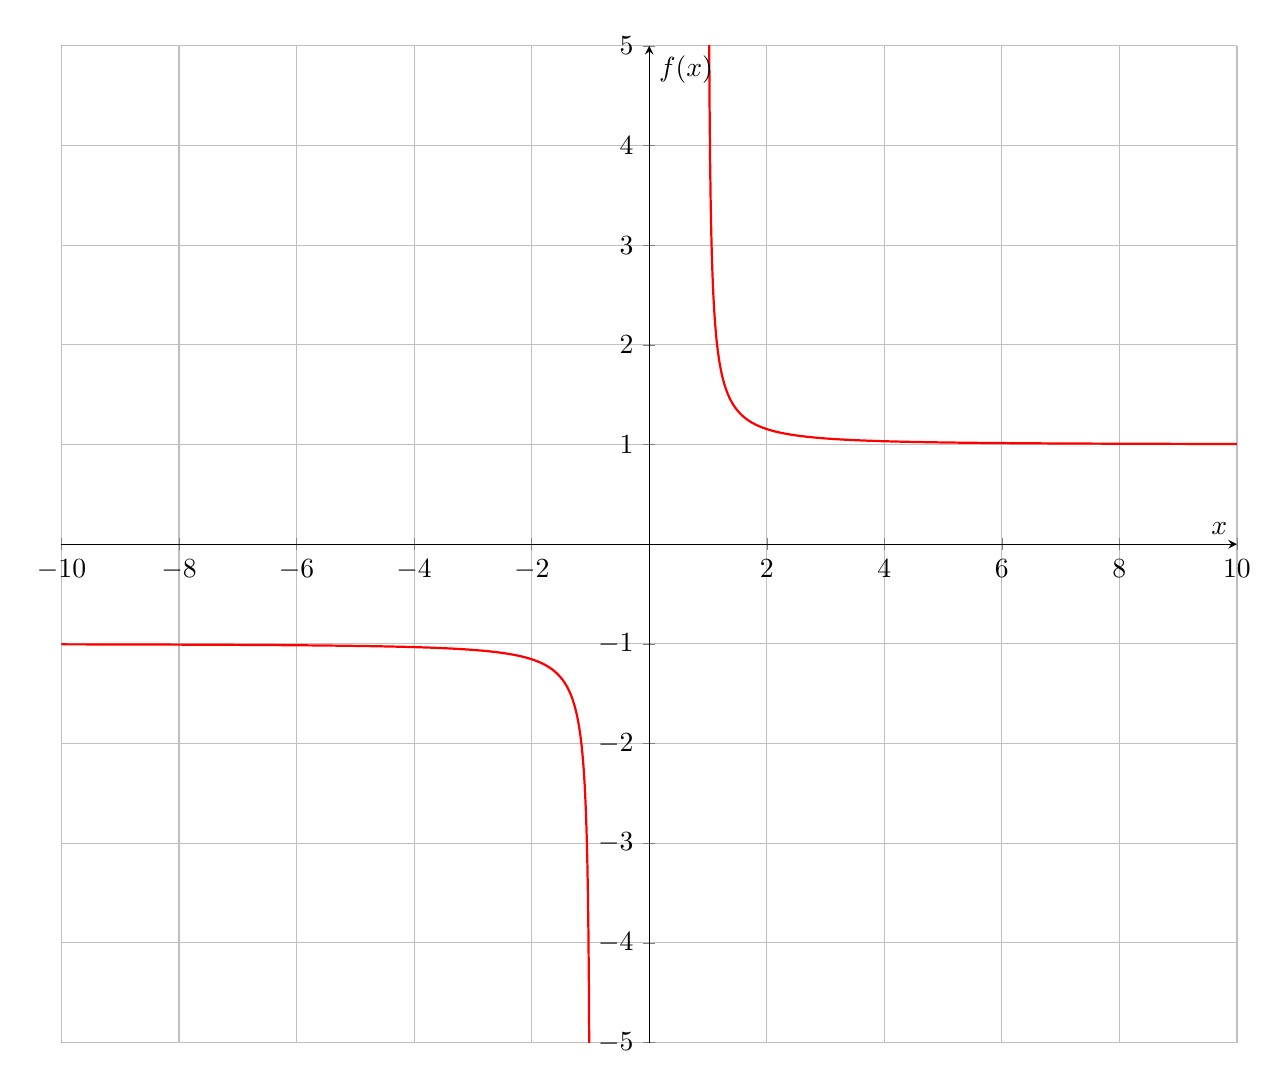
\begin{tikzpicture}
                        \begin{axis}[
                            axis lines = center,
                            xlabel = \(x\),
                            ylabel = {\(f(x)\)},
                            xmin = -10, xmax = 10,  % Adjusted the domain
                            ymin = -5, ymax = 5,  % Adjusted the range
                            samples = 1000,
                            domain = -5:10,  % Updated domain
                            grid = both,  % Optional: adds a grid
                            width = \linewidth,  % Optional: makes the plot fill the width
                        ]
                        \addplot [
                            domain=1:10, 
                            color = red,
                            thick,  % Optional: thickens the curve
                        ]
                        {x/sqrt(x^2-1)};
                        
                        \addplot [
                            domain=-10:-1, 
                            color = red,
                            thick,  % Optional: thickens the curve
                        ]
                        {x/sqrt(x^2-1)};
                        \end{axis}
                    \end{tikzpicture}
                \end{framed}
            \end{figure} 
        \end{enumerate}
        \setcounter{enumi}{32}
        \item Use the guidelines of this section to sketch the curve.
            \[y = \sin^3 x\]
        \begin{enumerate}
            \item Domain:\\
                Since this function is a trigonometric function. It will be continuous everywhere.\\
                The domain of this function is $(-\infty, \infty)$.
            \item Intercepts:
                \[f(0) = \sin^3 (0) = 0\]
                \[f(x) = \sin^3 (x) = 0\]
                \[x = n\pi \text{ with n is a integer.}\]
            The x-intercept is $n\pi \text{ with n is a integer.}$\\
            The y-intervals is 0.
            \newpage
            \item Symmetry:
                \[f(-x) = \sin^3(-x) = -\sin^3(x)\]
                \[f(-x) = -f(x)\]
            Hence, the function is odd.
            \item Asymptotes:\\
            The function doesn't have any asymptote since it is a trigonometric function.
            \item Intervals of Increase or Decrease:
                \[f'(x) = \sin^3(x)' = 3\sin^2(x)\cos(x) = 0\]
                \[\sin(x) = 0 \text{ or }\cos(x) = 0\]
                \[x = \frac{\pi}{2}n \text{ with n is a integer.}\]
                \begin{center}
                    \begin{tabular}{c c c c c c c c c c c c c}
                        $x$ & $-\infty$ & ... & 0 & ~ & $\pi/2$ & ~ & $\pi$ & ~ & $\pi 3/2$ & ... & $\infty$ \\ 
                        \hline 
                        $f^{\prime} (x)$ & ~ & ... & 0 & + & 0 & - & 0 & + & 0 & ... \\ 
                    \end{tabular}    
                \end{center}     
            The function repeated itself each $\frac{\pi}{2}$. 
            \item Local Maximum and Minimum Values:
                \[ -1 \leq \sin(x) \leq 1\]
                \[ (-1)^3 \leq \sin^3(x) \leq (1)^3\]
                \[ -1 \leq \sin^3(x) \leq 1\]
            Hence, the function local maximum is 1 and local minimum is -1.
            \item Concavity and Inflection Points:
                \[f''(x) = 3\sin^2(x)'\cos(x) + \cos(x)'3\sin^2(x)\]
                \[f''(x) = 6\sin(x)\cos^2(x) - 3\sin^3(x) = 0\]
                \[6\sin(x)\cos^2(x) = 3\sin^3(x)\]
                \[2 = \frac{\sin^2(x)}{\cos^2(x)}\]
                \[tan(x) = \sqrt{2}\]
                \[x = \tan^{-1}\sqrt{2} + n\pi \text{ with n is an integer.}\]
            The function is concave up in $(0, \tan^{-1}\sqrt{2})$ \\
            then concave down in $(\tan^{-1}\sqrt{2}, \tan^{-1}\sqrt{2} + \pi)$ and repeats itself.
            \newpage
            \item Sketch the graph:
            \begin{figure}[!h]
                \centering
                \begin{framed}
                    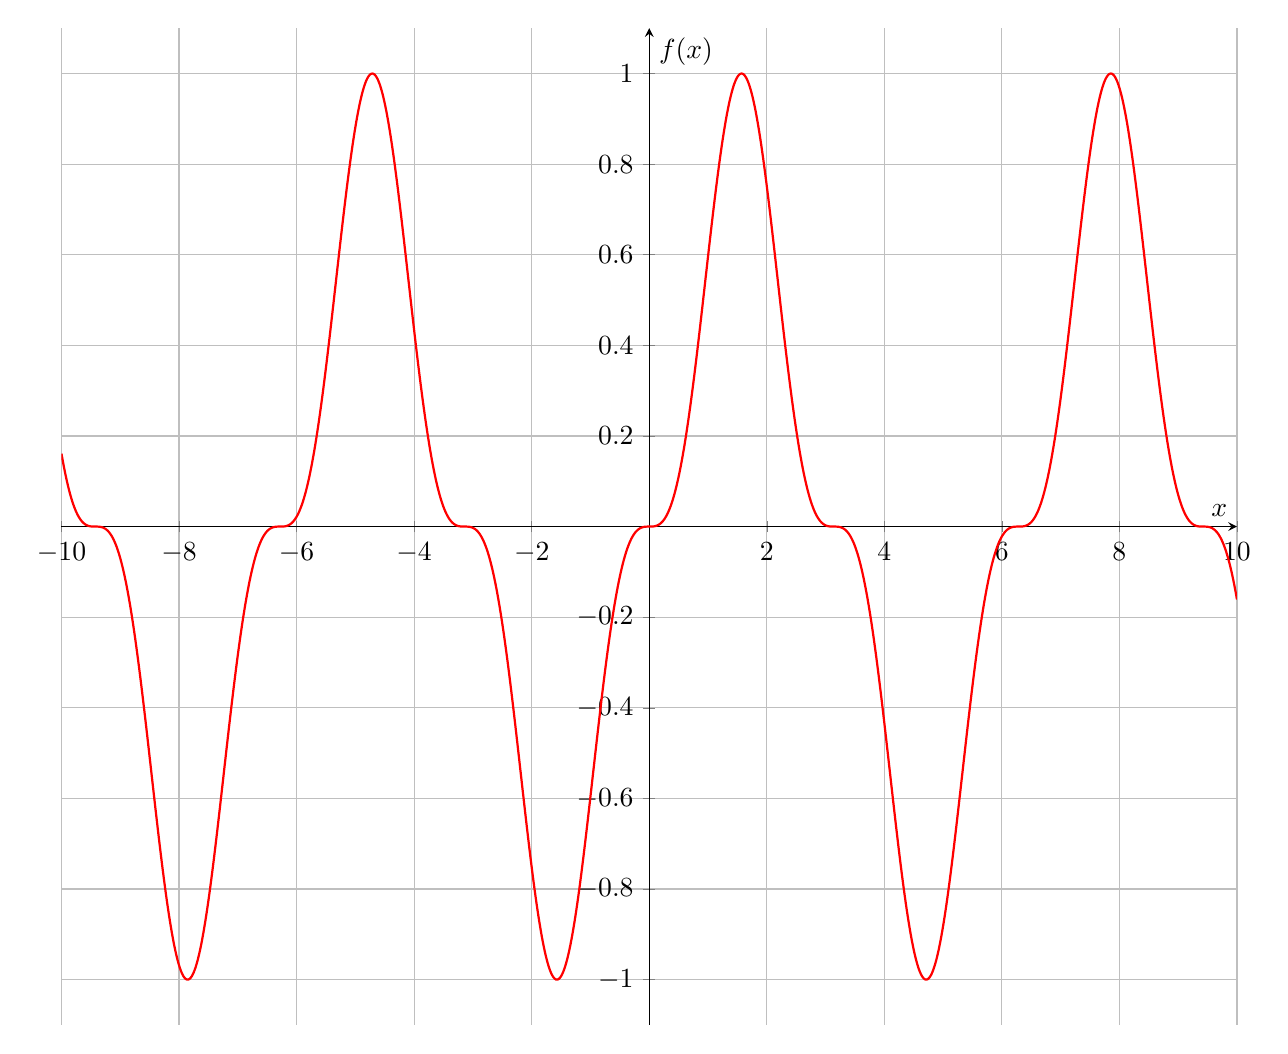
\begin{tikzpicture}
                        \begin{axis}[
                            axis lines = center,
                            xlabel = \(x\),
                            ylabel = {\(f(x)\)},
                            xmin = -10, xmax = 10,  % Domain for x
                            ymin = -1.1, ymax = 1.1,  % Range for y
                            samples = 10000,  % Number of samples for smoothness
                            grid = both,  % Adds grid lines
                            width = \linewidth,  % Fills the figure width
                        ]
                        \addplot [
                            domain=-10:10,
                            color = red,
                            thick,  % Thickens the curve
                        ]
                        {sin(deg(x))^3};  % Use deg() to convert from radians to degrees
                        \end{axis}
                    \end{tikzpicture}
                \end{framed}
            \end{figure}
        \end{enumerate}
        \setcounter{enumi}{40}
        \item The graph of a function $f$ is shown. (The dashed lines indicate horizontal asymptotes.) Find each of the following for the given function $g$.
            \begin{center}
                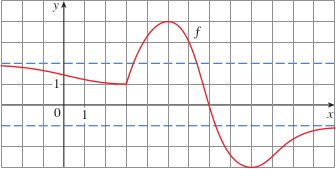
\includegraphics{img/img-1.png}
            \end{center}
            \[g(x) = \sqrt{f(x)}\]
            \begin{enumerate}
                \item The domains of $g$ and $g'$.\\
                    The domain of $g$ is $(-\infty, 7]$.
                    \[g'(x) = \frac{f'(x)}{2\sqrt{f(x)}}\]
                    The domain of $g'$ is $(-\infty, 3) \cup (3, 7)$.
                    \newpage
                \item The critical numbers of $g$.
                    \[g'(x) = \frac{f'(x)}{2\sqrt{f(x)}} = 0\]
                    \[f'(x) = 0\]
                    \[x = 3 \text{ or } x = 5\]
                \item The approximate value of $g'(6)$.
                    \[g'(6) = \frac{f'(6)}{2\sqrt{f(6)}} \approx \frac{-2}{4} = -\frac{1}{2}\]
                \item All vertical and horizontal asymptotes of $g$.
                    \[g(x) = \sqrt{f(x)}\]
                Because $f(x)$ has horizontal asymptotes f(x) = 2 and f(x) = -1. But f(x) = -1 is not defined for g(x).\\
                Therefore, $g(x) = \sqrt{f(x)} = \sqrt{2}$. Hence the horizontal asymptote of $g$ is $y = \sqrt{2}$.
            \end{enumerate}
            \setcounter{enumi}{52}
            \item Use the guidelines of this section to sketch the curve. In guideline $D$, find an equation of the slant asymptote.
                \[y = \frac{x^2}{x-1}\]
                \begin{enumerate}
                    \item Domain:
                        \[x - 1 \neq 0\]
                        \[x \neq 1\]
                    Hence the domain of the function is $(-\infty, 1) \cup (1, \infty)$.
                    \item Intercepts:
                        \[f(0) = \frac{0^2}{0-1} = 0\]
                        \[f(x) = \frac{x^2}{x-1} = 0\]
                        \[x = 0\]
                    Hence, the y-intercept is 0.
                    The x-intercept is 0.
                    \item Symmetry:
                        \[f(-x) = \frac{(-x)^2}{-x-1} = \frac{x^2}{-x-1}\]
                    Hence the function is not odd nor even.
                    \item Asymptotes:
                        \[\lim_{x \to 1^+} \frac{x^2}{x-1} = \infty\]
                        \[\lim_{x \to 1^-} \frac{x^2}{x-1} = -\infty\]
                        \[\lim_{x \to \infty} \frac{x^2}{x-1} = \lim_{x \to \infty} \frac{x}{1-1/x} = \infty\]
                        \[\lim_{x \to -\infty} \frac{x^2}{x-1} = -\infty\]
                        Hence, the function has vertical asymptotes x = 1.\\
                        The slant asymptote after doing long division is $y = x + 1$.
                    \item Intervals of Increase or Decrease:
                        \[f'(x) = \frac{(x^2)'(x-1) - (x-1)'(x^2)}{x-1}\]
                        \[f'(x) = \frac{2x(x-1) - (x^2)}{x-1}\]
                        \[f'(x) = \frac{2x^2- 2x - x^2}{x-1}\]
                        \[f'(x) = \frac{(x^2- 2x)}{x-1} = 0\]
                        \[x = 0 \text{ or } x = 2\]
                        \begin{center}
                            \begin{tabular}{c c c c c c c c c c c c}
                                $x$ & $-\infty$ & ~ & 0 & ~ & 1 & ~ & 2 & ~ & $\infty$ \\ 
                                \hline 
                                $f^{\prime} (x)$ & ~ & -- & 0 & + & $||$ & -- & 0 & + \\ 
                            \end{tabular}    
                        \end{center}
                        Hence, the function increases on the interval (0,1) and $(2,\infty)$.\\
                        The function decreases on the interval $(-\infty, 0)$ and (1,2).
                    \item Local Maximum and Minimum Values:\\
                    Local Minimum Values:    
                        \[f(0) = \frac{0^2}{0-1} = 0\]
                        \[f(2) = \frac{2^2}{2-1} = 4\]
                    \item Concavity and Inflection Points:
                        \[f''(x) = \frac{(x^2- 2x)'(x-1) - (x-1)'(x^2-2x)}{(x-1)^2}\]
                        \[f''(x) = \frac{(2x- 2)(x-1) - (x^2-2x)}{(x-1)^2}\]
                        \[f''(x) = \frac{2x^2 - 2x -2x + 2 - x^2 + 2x}{(x-1)^2}\]
                        \[f''(x) = \frac{x^2 - 2x + 2}{(x-1)^2} = 0\]
                        There is no solution for this function.
                        \begin{center}
                            \begin{tabular}{c c c c c c c c c c}
                                $x$ & $-\infty$ & ~ & 1 & ~ $\infty$ \\ 
                                \hline 
                                $f^{\prime\prime} (x)$ & ~ & -- & $||$ & +\\ 
                            \end{tabular}    
                        \end{center}
                        The function is concave up on the interval $(1, \infty)$.\\
                        The function is concave down on the interval $(-\infty, 1)$.
                    \item Sketch the graph:
                    \begin{figure}[!h]
                        \centering
                        \begin{framed}
                            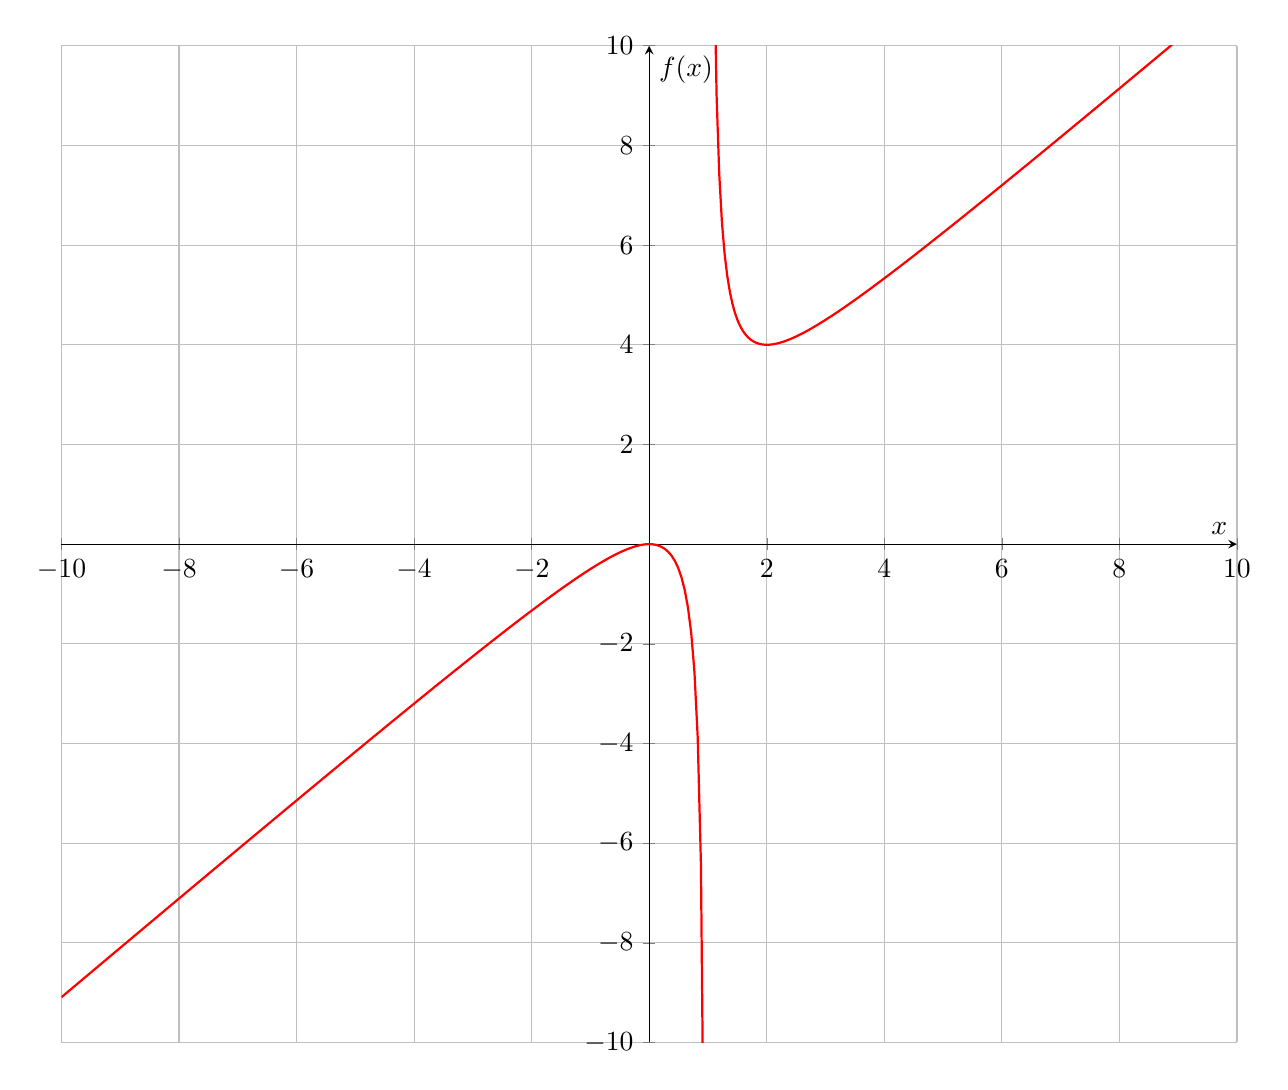
\begin{tikzpicture}
                                \begin{axis}[
                                    axis lines = center,
                                    xlabel = \(x\),
                                    ylabel = {\(f(x)\)},
                                    xmin = -10, xmax = 10,  % Domain for x
                                    ymin = -10, ymax = 10,  % Adjusted range for y to account for the function's behavior
                                    samples = 200,  % Number of samples for smoothness
                                    grid = both,  % Adds grid lines
                                    width = \linewidth,  % Fills the figure width
                                ]
                                \addplot [
                                    domain=-10:0.99,  % Left of the discontinuity
                                    color = red,
                                    thick,  % Thickens the curve
                                ]
                                {(x^2)/(x-1)};
                                
                                \addplot [
                                    domain=1.01:10,  % Right of the discontinuity
                                    color = red,
                                    thick,  % Thickens the curve
                                ]
                                {(x^2)/(x-1)};
                                
                                \end{axis}
                            \end{tikzpicture}
                        \end{framed}
                    \end{figure}
                \end{enumerate}
                \setcounter{enumi}{58}
                \item 
                Show that the curve $y = \sqrt{4x^2 + 9}$ has two slant asymptotes: $y = 2x$ and $y = --2x$. Use this fact to help sketch the curve.

\end{enumerate}

\end{document}